\section{Archimate 2.0}

Según  \cite{archimate2}, archimate es un lenguaje estandar utilizado por los arquitectos de software para modelar las necesidades de cada \textit{stakeholder}, dividiendo el contexto en el que se desenvuelve el software a desarrollar en tres capas: capa de negocio, capa de aplicación y capa de infraestructura.

\subsection{Capas de archimate}

A continuación serán descritas las tres capas definidas en el estandar archimate.

\subsubsection{Capa de negocio}

Esta capa envuelve todos los conceptos relacionados con la organización sobre la cual se aplicará el software a desarrollar, esto es, los roles, los servicios ofrecidos, los procesos, los productos y demás conceptos aplicados sobre su estructura y dinámica. Los artefactos de esta capa utilizados en el proyecto se enuncian en el cuadro \ref{tab:artefactos_capa_negocio}.

\begin{table}
  \caption{Artefactos de la capa de negocio}
  \label{tab:artefactos_capa_negocio}

  \begin{center}
  
  \textbf{Fuente:} \cite{archimate2}
  
  \resizebox{15cm}{!}{
  \begin{tabular}{|L{1cm}L{3cm}c|}
    \hline
    \multicolumn{1}{c}{Artefacto} & \multicolumn{1}{c}{Descripción} & \multicolumn{1}{c}{Notación} \\ 
    \hline
    \multicolumn{1}{c}{\textit{Actor de negocio (Business actor)}} & 
    \multicolumn{1}{c}{Ente (persona) organizacional quien cumple tareas en la organización} &  
    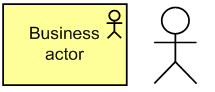
\includegraphics[width=7cm]{./imagenes/Archimate/businessactor.png}\\
    %\begin{figure}[!htb]
  	%	\begin{center}
    %		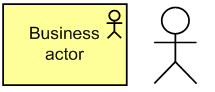
\includegraphics[width=11cm]{./imagenes/Archimate/businessactor.png}
    %		\label{fig:businessactor}
    %		\textbf{Fuente:}  \cite{archimate2}
  	%	\end{center}
	%\end{figure}  
	\hline
	\multicolumn{1}{c}{\textit{Colaboración de negocio (Business collaboration)}} & 
    \multicolumn{1}{c}{Rol que surge de la combinación de dos o más roles} &  
    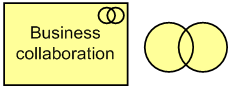
\includegraphics[width=7cm]{./imagenes/Archimate/businesscollaboration.png}\\
	\hline    
    \multicolumn{1}{c}{\textit{Rol de negocio (Business role)}} & 
    \multicolumn{1}{c}{Es un conjunto de responsabilidades que tiene asignado un actor. Dicho conjunto está definido por un solo concepto (nombre)} &  
    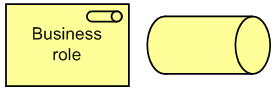
\includegraphics[width=7cm]{./imagenes/Archimate/businessrole.png}\\
    \hline
    \multicolumn{1}{c}{\textit{Proceso de negocio (Business process)}} & 
    \multicolumn{1}{c}{Agrupa comportamientos que se ejecutan como una serie de pasos} &  
    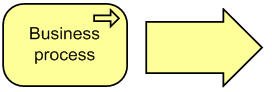
\includegraphics[width=7cm]{./imagenes/Archimate/businessprocess.png}\\
	\hline
	\multicolumn{1}{c}{\textit{Función de negocio (Business function)}} & 
    \multicolumn{1}{c}{Agrupa comportamientos que requieren una serie de competencias o recursos de negocio} &  
    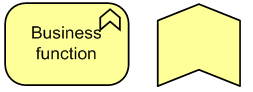
\includegraphics[width=7cm]{./imagenes/Archimate/businessfunction.png}\\
	\hline
	\multicolumn{1}{c}{\textit{Interacción de negocio (Business interaction)}} & 
    \multicolumn{1}{c}{Comportamientos realizados por colaboraciones de negocio} &  
    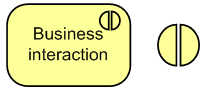
\includegraphics[width=7cm]{./imagenes/Archimate/businessinteraction.png}\\
	\hline
	\multicolumn{1}{c}{\textit{Evento de negocio (Business event)}} & 
    \multicolumn{1}{c}{Hecho que dispara un comportamiento (o grupo de comportamientos) en la organización} &  
    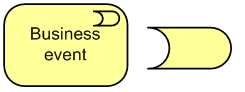
\includegraphics[width=7cm]{./imagenes/Archimate/businessevent.png}\\
	\hline
	\multicolumn{1}{c}{\textit{Servicio de negocio (Business service)}} & 
    \multicolumn{1}{c}{Servicio que cumple una necesidad del usuario} &  
    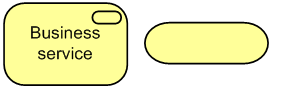
\includegraphics[width=7cm]{./imagenes/Archimate/businessservice.png}\\
	\hline
	\multicolumn{1}{c}{\textit{Producto (Product)}} & 
    \multicolumn{1}{c}{Agrupación de servicios que, definidos por un contrato, serán compartidos a clientes (tanto roles dentro de la organización como para clientes externos)} &  
    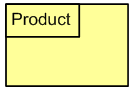
\includegraphics[width=7cm]{./imagenes/Archimate/businessproduct.png}\\
	\hline
  \end{tabular}
  }
    \end{center}
\end{table}

\subsubsection{Capa de aplicación} 

Esta capa cubre los conceptos relacionados con el modelamiento del sistema de información que soporta el negocio (la organización), previamente modelado en la capa de negocio. Los artefactos de esta capa utilizados en el proyecto se enuncian en el cuadro \ref{tab:artefactos_capa_aplicacion}.

\begin{table}
  \caption{Artefactos de la capa de aplicación}
  \label{tab:artefactos_capa_aplicacion}

  \begin{center}
  
  \textbf{Fuente:} \cite{archimate2}
  
  \resizebox{15cm}{!}{
  \begin{tabular}{|L{1cm}L{3cm}c|}
    \hline
    \multicolumn{1}{c}{Artefacto} & \multicolumn{1}{c}{Descripción} & \multicolumn{1}{c}{Notación} \\ 
    \hline
    \multicolumn{1}{c}{\textit{Componente de aplicación (Application component)}} & 
    \multicolumn{1}{c}{Unidad de software} &  
    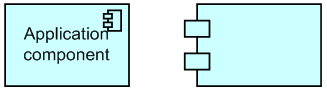
\includegraphics[width=7cm]{./imagenes/Archimate/applicationcomponent.png}\\
	\hline
	\multicolumn{1}{c}{\textit{Colaboración de aplicación (Application collaboration)}} & 
    \multicolumn{1}{c}{Colaboración entre dos o más componentes de aplicación para realizar una tarea que necesita de cada uno de ellos} &  
    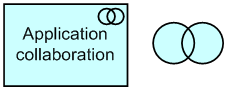
\includegraphics[width=7cm]{./imagenes/Archimate/applicationcollaboration.png}\\
	\hline    
    \multicolumn{1}{c}{\textit{Función de aplicación (Application function)}} & 
    \multicolumn{1}{c}{Agrupa comportamientos que pueden ser automatizados por un componente de aplicación} &  
    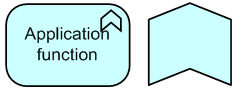
\includegraphics[width=7cm]{./imagenes/Archimate/applicationfunction.png}\\
    \hline
    \multicolumn{1}{c}{\textit{Interacción de aplicación (Application interaction)}} & 
    \multicolumn{1}{c}{Agrupa comportamientos que pueden ser automatizados por una colaboración de aplicación} &  
    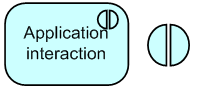
\includegraphics[width=7cm]{./imagenes/Archimate/applicationinteraction.png}\\
	\hline
	\multicolumn{1}{c}{\textit{Servicio de aplicación (Application service)}} & 
    \multicolumn{1}{c}{Un servicio que expone las funcionalidades automatizadas ofrecidas} &  
    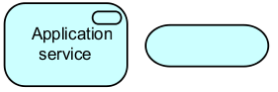
\includegraphics[width=7cm]{./imagenes/Archimate/applicationservice.png}\\
	\hline
  \end{tabular}
  }
    \end{center}
\end{table}

\subsubsection{Capa de infraestructura}

Capa que modela el posicionamiento físico del software a utilizar, así como también los requerimientos que este tiene para su funcionamiento a nivel físico (servidores, redes, nodos, etc.). Los artefactos de esta capa utilizados en el proyecto se enuncian en el cuadro \ref{tab:artefactos_capa_infraestructura}.


\begin{table}
  \caption{Artefactos de la capa de infraestructura}
  \label{tab:artefactos_capa_infraestructura}

  \begin{center}
  
  \textbf{Fuente:} \cite{archimate2}
  
  \resizebox{15cm}{!}{
  \begin{tabular}{|L{1cm}L{3cm}c|}
    \hline
    \multicolumn{1}{c}{Artefacto} & \multicolumn{1}{c}{Descripción} & \multicolumn{1}{c}{Notación} \\ 
    \hline
    \multicolumn{1}{c}{\textit{Nodo (Node)}} & 
    \multicolumn{1}{c}{Recurso computacional que agrupa artefactos almacenables o desplegables para ser ejecutados} &  
    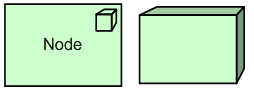
\includegraphics[width=7cm]{./imagenes/Archimate/technologynode.png}\\
	\hline
	\multicolumn{1}{c}{\textit{Dispositivo (Device)}} & 
    \multicolumn{1}{c}{Hardware que contiene elementos software para ser ejecutados} &  
    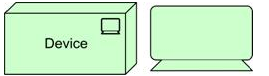
\includegraphics[width=7cm]{./imagenes/Archimate/technologydevice.png}\\
	\hline    
    \multicolumn{1}{c}{\textit{Red (Network)}} & 
    \multicolumn{1}{c}{Medio de comunicación entre dos o más nodos o dispositivos} &  
    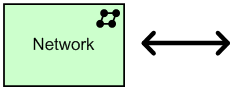
\includegraphics[width=7cm]{./imagenes/Archimate/technologynetwork.png}\\
    \hline
    \multicolumn{1}{c}{\textit{Sistema de software (System software)}} & 
    \multicolumn{1}{c}{Software sobre el cual se realizan (o representan) los artefactos (componentes de aplicación) desplegables} &  
    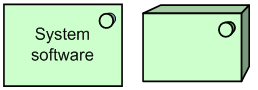
\includegraphics[width=7cm]{./imagenes/Archimate/technologyswsystem.png}\\
	\hline
	\multicolumn{1}{c}{\textit{Servicio de infraestructura (Infraestructure service)}} & 
    \multicolumn{1}{c}{Servicios que agrupan funcionalidades prestadas por nodos} &  
    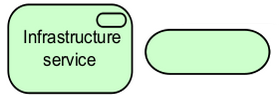
\includegraphics[width=7cm]{./imagenes/Archimate/technologyservice.png}\\
	\hline
  \end{tabular}
  }
    \end{center}
\end{table}

\subsection{Relaciones}

Las relaciones, en archimate, son aquellas conexiones existentes entre dos artefactos. Hay tres tipos de relaciones en archimate: relaciones estructurales, relaciones dinámicas y otras que no caben en las dos últimas.

\begin{itemize}

\item \textbf{Relaciones estructurales}: Estas relaciones modelan la coherencia estructural generada por la unión estructural de todos los artefactos de la arquitectura. En el cuadro \ref{tab:relaciones_estructurales} se hace un sumario de las relaciones estructurales utilizadas para unir los artefactos utilizados en el presente proyecto:

\begin{table}
  \caption{Relaciones estructurales}
  \label{tab:relaciones_estructurales}

  \begin{center}
  
  \textbf{Fuente:} \cite{archimate2}
  
  \resizebox{15cm}{!}{
  \begin{tabular}{|L{1cm}L{3cm}c|}
    \hline
    \multicolumn{1}{c}{Relación} & \multicolumn{1}{c}{Descripción} & \multicolumn{1}{c}{Notación} \\ 
    \hline
    \multicolumn{1}{c}{\textit{Asociación (Association)}} & 
    \multicolumn{1}{c}{Cumple la función de asociar dos artefactos que no tienen una relación más específica} &  
    
\includegraphics[width=7cm]{./imagenes/Archimate/relassociation.png}\\
	\hline
	\multicolumn{1}{c}{\textit{Usado por (Used by)}} & 
    \multicolumn{1}{c}{Modela el acceso a servicios o interfaces. El acceso a interfaces solo puede ser realizado por artefactos estructurales y a los servicios solo los artefactos comportamentales} &  
    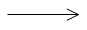
\includegraphics[width=7cm]{./imagenes/Archimate/relusedby.png}\\
	\hline    
    \multicolumn{1}{c}{\textit{Realización (Realization)}} & 
    \multicolumn{1}{c}{Une un artefacto abstracto con otro más concreto que lo realiza} &  
    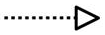
\includegraphics[width=7cm]{./imagenes/Archimate/relrealization.png}\\
    \hline
    \multicolumn{1}{c}{\textit{Asignación (Assignment)}} & 
    \multicolumn{1}{c}{Une artefactos con aquellos que, por obligación, deben utilizar otros (por ejemplo, un rol con una función de negocio)} &  
    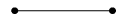
\includegraphics[width=7cm]{./imagenes/Archimate/relassignment.png}\\
	\hline
	\multicolumn{1}{c}{\textit{Agregación (Aggregation)}} & 
    \multicolumn{1}{c}{Es la composición de un artefacto por otros. Esta composición no es destructiva, es decir, si el artefacto que es compuesto deja de existir, los otros seguirán existiendo} &  
    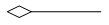
\includegraphics[width=7cm]{./imagenes/Archimate/relaggregation.png}\\
	\hline
	\multicolumn{1}{c}{\textit{Composición (Composition)}} & 
    \multicolumn{1}{c}{Es la composición de un artefacto por otros. Esta composición es destructiva, es decir, si el artefacto que es compuesto deja de existir, los otros también} &  
    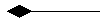
\includegraphics[width=7cm]{./imagenes/Archimate/relcomposition.png}\\
	\hline
  \end{tabular}
  }
    \end{center}
\end{table}

\item \textbf{Relaciones dinámicas}: Esta relación expresa una unión temporal entre dos artefactos donde, posiblemente, uno de los artefactos use a otro para cumplir un fin específico.En el cuadro \ref{tab:relaciones_dinamicas} se hace un sumario de las relaciones dinámicas utilizadas para unir los artefactos utilizados en el presente proyecto.

\begin{table}
  \caption{Relaciones dinámicas}
  \label{tab:relaciones_dinamicas}

  \begin{center}
  
  \textbf{Fuente:} \cite{archimate2}
  
  \resizebox{15cm}{!}{
  \begin{tabular}{|L{1cm}L{3cm}c|}
    \hline
    \multicolumn{1}{c}{Relación} & \multicolumn{1}{c}{Descripción} & \multicolumn{1}{c}{Notación} \\ 
    \hline
    \multicolumn{1}{c}{\textit{Flujo (Flow)}} & 
    \multicolumn{1}{c}{Describe intercambios de información entre artefactos comportamentales} &  
    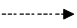
\includegraphics[width=7cm]{./imagenes/Archimate/relflow.png}\\
	\hline
	\multicolumn{1}{c}{\textit{Disparador (Triggering)}} & 
    \multicolumn{1}{c}{Describe la relación temporal o factual entre 2 artefactos comportamentales} &  
    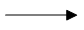
\includegraphics[width=7cm]{./imagenes/Archimate/reltriggering.png}\\
	\hline
  \end{tabular}
  }
    \end{center}
\end{table}

\item \textbf{Otras relaciones}: En el cuadro \ref{tab:otras_relaciones} se hace un sumario de las relaciones que no pueden ser incluidas en las dinámicas o en las estructurales y que son utilizadas para unir los artefactos utilizados en el presente proyecto.

\begin{table}
  \caption{Otras relaciones}
  \label{tab:otras_relaciones}

  \begin{center}
  
  \textbf{Fuente:} \cite{archimate2}
  
  \resizebox{15cm}{!}{
  \begin{tabular}{|L{1cm}L{3cm}c|}
    \hline
    \multicolumn{1}{c}{Relación} & \multicolumn{1}{c}{Descripción} & \multicolumn{1}{c}{Notación} \\ 
    \hline
    \multicolumn{1}{c}{\textit{Unión (Junction)}} & 
    \multicolumn{1}{c}{Cumple la función de asociar dos artefactos que no tienen una relación más específica} &  
    
\includegraphics[width=7cm]{./imagenes/Archimate/reljunction.png}\\
	\hline
	\multicolumn{1}{c}{\textit{Especialización (Specialization)}} & 
    \multicolumn{1}{c}{Indica la especialización de un artefacto tomando otro como referencia} &  
    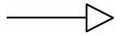
\includegraphics[width=7cm]{./imagenes/Archimate/relspecialization.png}\\
	\hline
  \end{tabular}
  }
    \end{center}
\end{table}

\end{itemize}

\subsection{Vistas archimate}

Debido a la existencia de diferentes stakeholders en el desarrollo de software, se hace necesario mostrar aquella parte de la arquitectura que cierto stakeholder necesita para tener una vista entera del negocio, el sistema de información o la infraestructura, o bien una combinación de ellos.

Archimate utiliza el concepto de “vistas” como la segmentación de la arquitectura en vistas que conciernen al stakeholder que quiera echar un vistaso a la arquitectura, escondiendo detalles de la arquitectura que no le interesan a este.

En los cuadros \ref{tab:introductory_viewpoint} a \ref{tab:product_viewpoint} se pueden ver las vistas utilizadas, con su descripci´on y su metamodelo.

\begin{table}
  \caption{Punto de vista introductorio}
  \label{tab:introductory_viewpoint}

  \begin{center}
  
  \textbf{Fuente:} \cite{archimate2}
  
  \resizebox{15cm}{!}{
  \begin{tabular}{|L{1cm}L{3cm}|}
    \hline
    \multicolumn{1}{c}{Punto de vista} & 
    \multicolumn{1}{c}{Punto de vista introductorio (introductory viewpoint)} \\ 
    \hline
    \multicolumn{1}{c}{Stakeholders} & 
    \multicolumn{1}{c}{Arquitectos empresariales y gerentes generales} \\ 
    \hline
    \multicolumn{1}{c}{Concerns} & 
    \multicolumn{1}{c}{Da un panorama de los cambios, representaciones o adiciones del o a la organización. Ayuda a la toma de decisiones} \\ 
    \hline
    \multicolumn{1}{c}{Propósito} & 
    \multicolumn{1}{c}{Diseñar, decidir e informar} \\ 
    \hline
    \multicolumn{1}{c}{Capas} & 
    \multicolumn{1}{c}{Negocio, aplicación e infraestructura} \\ 
    \hline
    \multicolumn{1}{c}{Metamodelo} &
    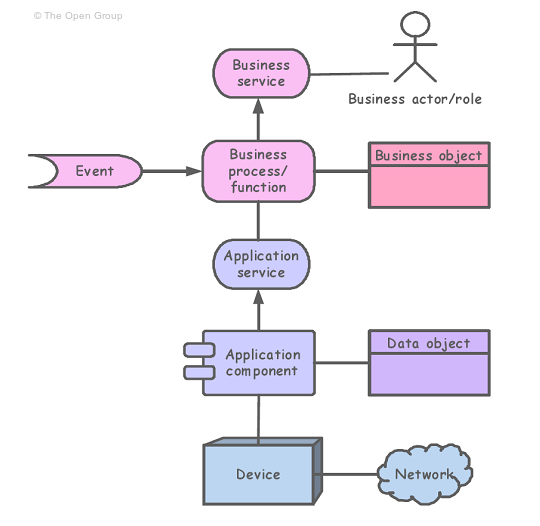
\includegraphics[width=7cm]{./imagenes/Archimate/introductoryviewpoint.png}\\
	\hline
  \end{tabular}
  }
    \end{center}
\end{table}

\begin{table}
  \caption{Punto de vista en capas}
  \label{tab:layered_viewpoint}

  \begin{center}
  
  \textbf{Fuente:} \cite{archimate2}
  
  \resizebox{15cm}{!}{
  \begin{tabular}{|L{1cm}L{3cm}|}
    \hline
    \multicolumn{1}{c}{Punto de vista} & 
    \multicolumn{1}{c}{Punto de vista en capas (layered viewpoint)} \\ 
    \hline
    \multicolumn{1}{c}{Stakeholders} & 
    \multicolumn{1}{c}{Arquitectos de dominio, infraestructura, procesos, aplicación y negocio} \\ 
    \hline
    \multicolumn{1}{c}{Concerns} & 
    \multicolumn{1}{c}{Impacto del cambio, flexibilidad, reducción de la complejidad y consistencia} \\ 
    \hline
    \multicolumn{1}{c}{Propósito} & 
    \multicolumn{1}{c}{Diseñar, decidir e informar} \\ 
    \hline
    \multicolumn{1}{c}{Capas} & 
    \multicolumn{1}{c}{Negocio, aplicación e infraestructura} \\ 
    \hline
    \multicolumn{1}{c}{Metamodelo} &
    \multicolumn{1}{c}{Se usan los artefactos y relaciones de todas las capas, seg´un se considere pertinente}\\
	\hline
  \end{tabular}
  }
    \end{center}
\end{table}

\begin{table}
  \caption{Punto de vista de funci´on}
  \label{tab:business_function_viewpoint}

  \begin{center}
  
  \textbf{Fuente:} \cite{archimate2}
  
  \resizebox{15cm}{!}{
  \begin{tabular}{|L{1cm}L{3cm}|}
    \hline
    \multicolumn{1}{c}{Punto de vista} & 
    \multicolumn{1}{c}{Punto de vista de funci´on (business function viewpoint)} \\ 
    \hline
    \multicolumn{1}{c}{Stakeholders} & 
    \multicolumn{1}{c}{Organización, arquitectos de proceso y de dominio} \\ 
    \hline
    \multicolumn{1}{c}{Concerns} & 
    \multicolumn{1}{c}{Identificación de competencias, identificación de actividades principales y reducción de complejidad} \\ 
    \hline
    \multicolumn{1}{c}{Propósito} & 
    \multicolumn{1}{c}{Diseño} \\ 
    \hline
    \multicolumn{1}{c}{Capas} & 
    \multicolumn{1}{c}{Negocio} \\ 
    \hline
    \multicolumn{1}{c}{Metamodelo} &
    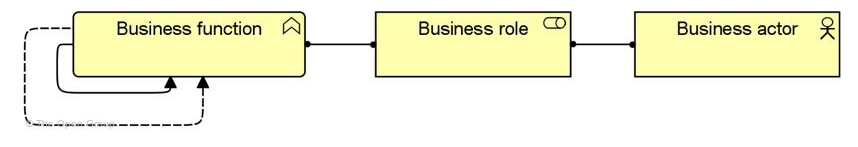
\includegraphics[width=7cm]{./imagenes/Archimate/businessfunctionviewpoint.png}\\
	\hline
  \end{tabular}
  }
    \end{center}
\end{table}

\begin{table}
  \caption{Punto de vista de proceso}
  \label{tab:business_process_viewpoint}

  \begin{center}
  
  \textbf{Fuente:} \cite{archimate2}
  
  \resizebox{15cm}{!}{
  \begin{tabular}{|L{1cm}L{3cm}|}
    \hline
    \multicolumn{1}{c}{Punto de vista} & 
    \multicolumn{1}{c}{Punto de vista de proceso (business process viewpoint)} \\ 
    \hline
    \multicolumn{1}{c}{Stakeholders} & 
    \multicolumn{1}{c}{Gerentes operacionales, aquitectos de dominio y de proceso} \\ 
    \hline
    \multicolumn{1}{c}{Concerns} & 
    \multicolumn{1}{c}{Estructura del proceso de negocio, consistencia y completitud así como también responsabilidades} \\ 
    \hline
    \multicolumn{1}{c}{Propósito} & 
    \multicolumn{1}{c}{Diseño} \\ 
    \hline
    \multicolumn{1}{c}{Capas} & 
    \multicolumn{1}{c}{Negocio y aplicación} \\ 
    \hline
    \multicolumn{1}{c}{Metamodelo} &
    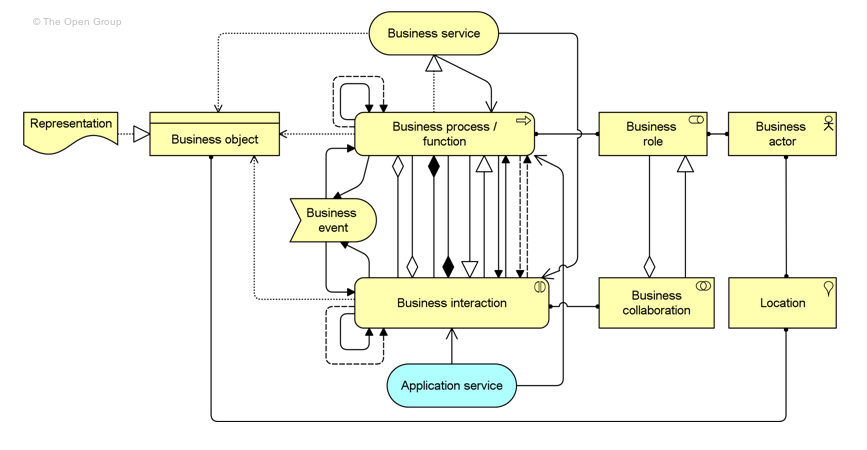
\includegraphics[width=7cm]{./imagenes/Archimate/businessprocessviewpoint.png}\\
	\hline
  \end{tabular}
  }
    \end{center}
\end{table}

\begin{table}
  \caption{Punto de vista de uso de aplicación}
  \label{tab:application_usage_viewpoint}

  \begin{center}
  
  \textbf{Fuente:} \cite{archimate2}
  
  \resizebox{15cm}{!}{
  \begin{tabular}{|L{1cm}L{3cm}|}
    \hline
    \multicolumn{1}{c}{Punto de vista} & 
    \multicolumn{1}{c}{Punto de vista de uso de aplicación (Application usage viewpoint)} \\ 
    \hline
    \multicolumn{1}{c}{Stakeholders} & 
    \multicolumn{1}{c}{Arquitectos de proceso, arquitectos de negocio, arquitectos de aplicación y gerentes operacionales} \\ 
    \hline
    \multicolumn{1}{c}{Concerns} & 
    \multicolumn{1}{c}{Competencia y completitud, reducción de la complejidad} \\ 
    \hline
    \multicolumn{1}{c}{Propósito} & 
    \multicolumn{1}{c}{Diseño y decisión} \\ 
    \hline
    \multicolumn{1}{c}{Capas} & 
    \multicolumn{1}{c}{Negocio y aplicación} \\ 
    \hline
    \multicolumn{1}{c}{Metamodelo} &
    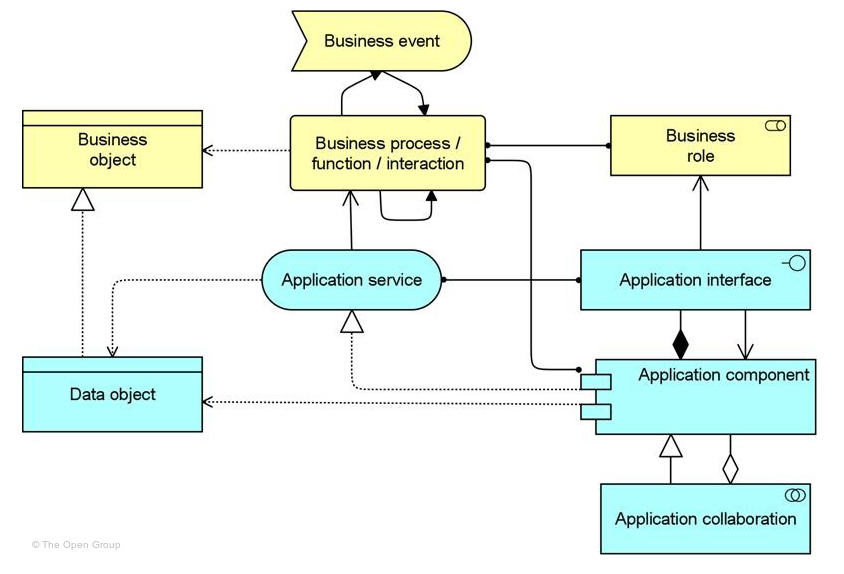
\includegraphics[width=7cm]{./imagenes/Archimate/applicationusageviewpoint.png}\\
	\hline
  \end{tabular}
  }
    \end{center}
\end{table}

\begin{table}
  \caption{Punto de vista de producto}
  \label{tab:product_viewpoint}

  \begin{center}
  
  \textbf{Fuente:} \cite{archimate2}
  
  \resizebox{15cm}{!}{
  \begin{tabular}{|L{1cm}L{3cm}|}
    \hline
    \multicolumn{1}{c}{Punto de vista} & 
    \multicolumn{1}{c}{Punto de vista de producto (Product viewpoint)} \\ 
    \hline
    \multicolumn{1}{c}{Stakeholders} & 
    \multicolumn{1}{c}{Desarrolladores de producto, gerentes de producto y de proceso, también los arquitectos de dominio} \\ 
    \hline
    \multicolumn{1}{c}{Concerns} & 
    \multicolumn{1}{c}{Desarrollo de producto y muestra del valor ofrecido por los productos de la organización} \\ 
    \hline
    \multicolumn{1}{c}{Propósito} & 
    \multicolumn{1}{c}{Diseño y decisión} \\ 
    \hline
    \multicolumn{1}{c}{Capas} & 
    \multicolumn{1}{c}{Negocio y aplicación} \\ 
    \hline
    \multicolumn{1}{c}{Metamodelo} & \\
    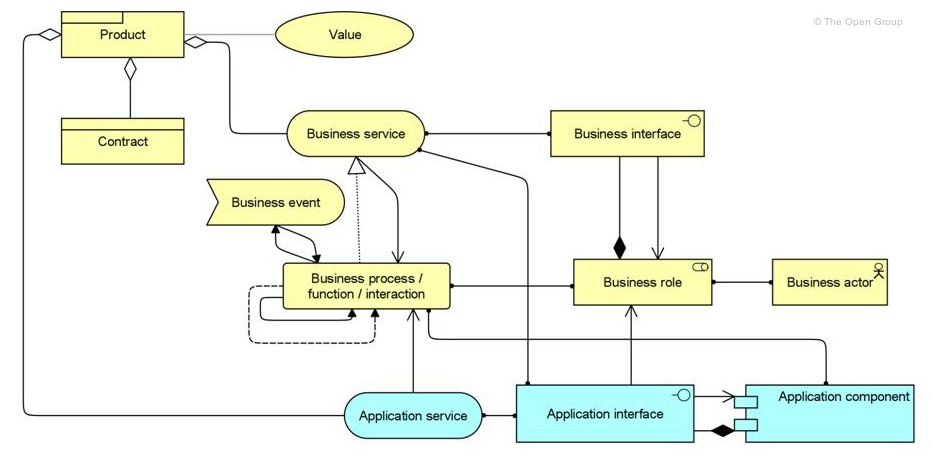
\includegraphics[width=7cm]{./imagenes/Archimate/productviewpoint.png}\\
	\hline
  \end{tabular}
  }
    \end{center}
\end{table}